%
% File acl2014.tex
%
% Contact: giovanni.colavizza@epfl.ch
%%
%% Based on the style files for ACL-2013, which were, in turn,
%% Based on the style files for ACL-2012, which were, in turn,
%% based on the style files for ACL-2011, which were, in turn, 
%% based on the style files for ACL-2010, which were, in turn, 
%% based on the style files for ACL-IJCNLP-2009, which were, in turn,
%% based on the style files for EACL-2009 and IJCNLP-2008...

%% Based on the style files for EACL 2006 by 
%%e.agirre@ehu.es or Sergi.Balari@uab.es
%% and that of ACL 08 by Joakim Nivre and Noah Smith

\documentclass[a4paper,11pt]{article}
\usepackage[utf8]{inputenc}
\usepackage{acl2014}
\usepackage{times}
\usepackage{hyperref}
\usepackage{latexsym}
\usepackage{graphicx}

\providecommand{\tightlist}{%
  \setlength{\itemsep}{0pt}\setlength{\parskip}{0pt}}
%\setlength\titlebox{5cm}

% You can expand the titlebox if you need extra space
% to show all the authors. Please do not make the titlebox
% smaller than 5cm (the original size); we will check this
% in the camera-ready version and ask you to change it back.


\title{Impact of Conflicts on African Civilian Population}

\author{Hrvoje Bušić \\
  \small{\tt hrvoje.busic@epfl.ch} \\\And
  Domenica Verbaro\\
  \small{\tt domenica.verbaro@epfl.ch} \\\And
Joey Zenhäusern\\
\small{\tt joey.zenhausern@epfl.ch} \\}

\date{}

\begin{document}
\maketitle
\begin{abstract}
The Uppsala conflict data set documents in detail frequency and nature of violent events occurring in the world. We are extending the data set with information about the Human Development Index and Freedom House scores measuring civil liberties, while conducting robust analysis on the impact that violent events have had on the African civilian population.
\end{abstract}

\section{Introduction}

The age of information makes it seem as though conflict and wars are, and always will be, ever growing part of our lives. We often feel overwhelmed by the amount and scope of information that is accessible and directed towards us, in turn rendering us indifferent to the consequences and casualties of the war.

Civilians are the greatest casualty of any war, and casualties are not always measured in body count. Civil liberties and political freedoms are and should be enjoyed by the people from all around the world, and conflicts always bring changes to freedom of expression, for better or worse.

In this project we will focus on the continent of Africa, which we feel is underreported in the context of occurring conflicts and casualties. We will utilize UDCP data set documenting individual events of organized violence, empowered by the Freedom House `Freedom in the World' yearly surveys and the Human Development Index as measured by the UN.

\section{Specification of regions and country
names}

Throughout this report, we will observe the African continent through its
regions as defined by the United Nations' geoscheme for Africa~\cite{UNGeoscheme}. This geoscheme is used by the UN and
maintained by the UNSD department for statistical purposes, and defines
five regions as depicted in Figure~\ref{fig:regions}.
\begin{figure}[ht!]
    \centering
    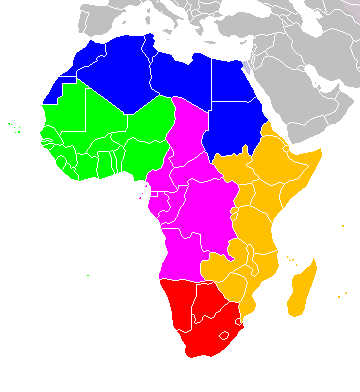
\includegraphics[width=0.2\textwidth]{images/Africa-regions.png}
    \caption{\footnotesize{UN Geoscheme: North (blue), East (yellow), South (red), Central (pink), West (green)\label{fig:regions}}}
\end{figure}

\section{UCDP dataset}

Uppsala Conflict Data Program's georeferenced event dataset \cite{Sundberg:13},
Global Version 17.1 \cite{Codebook2017}, is the central dataset used in our project.
The dataset covers individual events of organized violence --- phenomena of
lethal violence occurring at a given time and place.

This project makes use of the events which ocurred in the African region
throughout the period of 26 years (1990--2015), or roughly 35,437 events.

\section{Freedom House dataset}

Freedom House is a U.S.-based U.S. Government-funded non-governmental
organization (NGO) that conducts research and advocacy on democracy,
political freedom, and human rights.

The Organisation's reports on the state of country's political freedoms and
civil liberties form our second dataset.
We will focus our attention on data
which contains information about political freedom and civil liberties
scores for individual countries throughout the period of 1990--2015.

Political rights and civil liberties are measured on a one-to-seven
scale, with one representing the highest degree of freedom and seven the
lowest.

\section{Human Development Index}

The Human Development Index (HDI) is a composite statistic (composite
index) of life expectancy, education, and per capita income indicators,
which are used to rank countries into four tiers of human development. A
country scores higher HDI when the lifespan is higher, the education
level is higher, and the GDP per capita is higher.

The Human Development Index is a value in the range ${[}0,1{]}$, with 1 designating
the best possible value.

\section{Findings}

\subsection{North Africa}
\begin{figure}[ht!]
    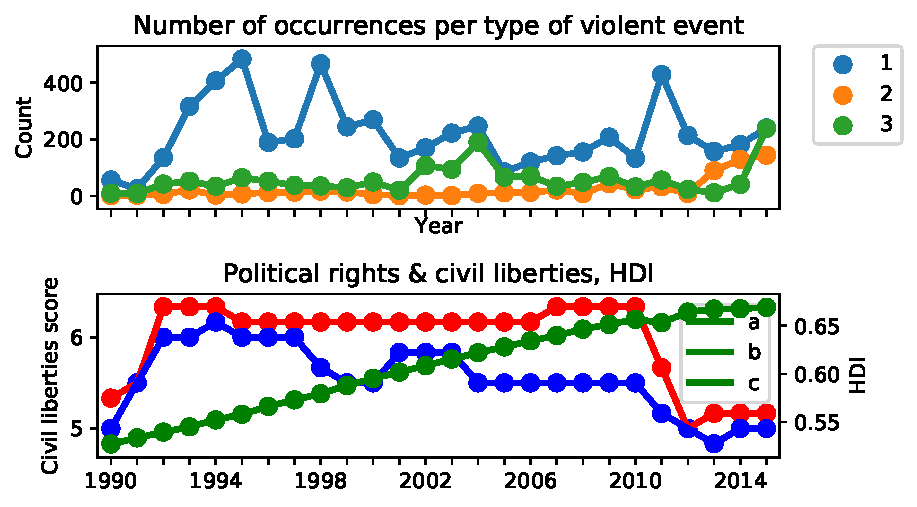
\includegraphics[width=0.50\textwidth]{images/na.pdf}
    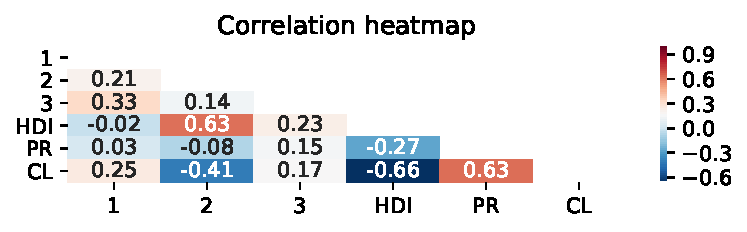
\includegraphics[width=0.50\textwidth]{images/na_corr.pdf}
\end{figure}
Throughout the early 90s Algeria is the main contributor of conflict in terms of number of conflicts, due to the Algerian Civil War, which spans more than a decade from 1991 to 2002. The largest contributor by number of deaths is Sudan, which also experiences a civil war in the timespan from 1983 to 2005. In this timeframe, political rights and civil liberties remain poor, but interestingly the HDI is steadily increasing, seemingly unaffected by any major conflict in the region.

Violence events of type 1 and 3 do not seem to have much effect on our indicator variables, judging by the low correlation scores, but violence events of type 2 appear to have some connection to civil liberty and HDI, albeit not the one expected. In both cases, the correlation is exactly opposite to what you would expect: A high number of type 2 violence is positively correlated with HDI, and negatively correlated with the civil liberty score. In the case of HDI this might simply be coincidence, given that the development of the metric is so stable. But regarding the civil liberty score there is an interesting possible interpretation: Civil liberty often has to be fought for. Looking at the period following the Arab Spring between 2010 and 2015 yields further evidence for this idea. A peak in violence is followed by an improvement in civil liberties as well as political rights.

\subsection{East Africa}
\begin{figure}[ht!]
    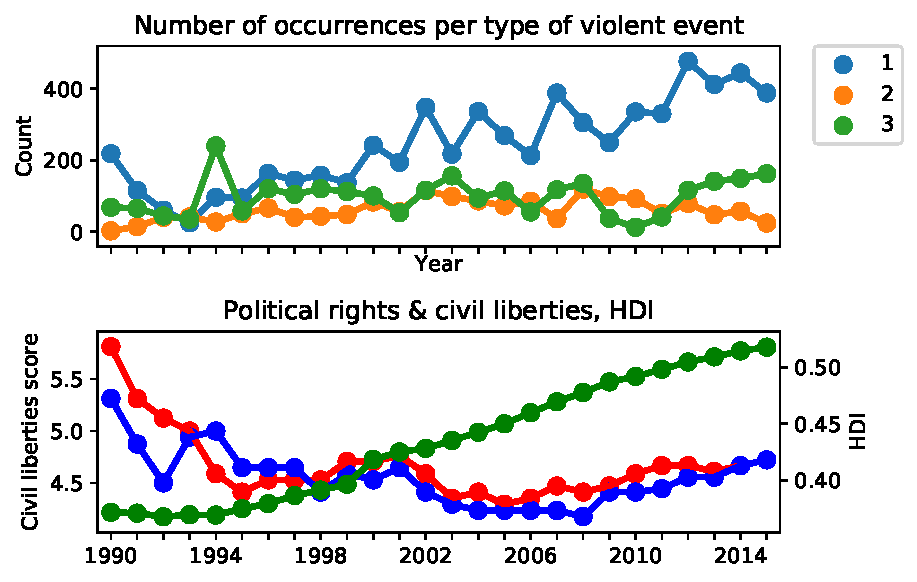
\includegraphics[width=0.50\textwidth]{images/ea.pdf}
    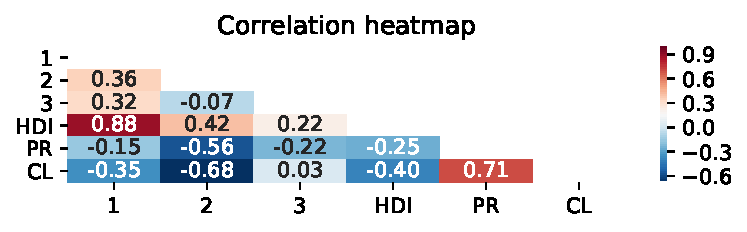
\includegraphics[width=0.50\textwidth]{images/ea_corr.pdf}
\end{figure}
We can make a similar observation for East Africa as for North Africa: Violence and HDI are positively correlated while violence and political rights or civily liberty are negatively correlated. This time the strongest positive correlation is between violence of type 1 and HDI\@. As before, the HDI on average appears to be a reliably growing metric, while civil liberty and political rights have been improving right until the year 2008, after which they started deteriorating again.

One thing to take into consideration is that Rwanda skews the numbers heavily in 1994, owing to the Rwandan genocide taking place in that year. Remarkably, Rwanda made a steep recovery following this tragic event, we can see their HDI rising from less than 0.2 to nearly 0.5 in the years following 1994, while the occurence of violent events is steadily declining.

The the recent negative regional trend in civily liberty and political rights is due to the fact that many countries in the region have been experiencing conflicts and political instabilities. Notable examples are Eritrea and Ethiopia who, following the Eritrean-Ethiopian War from 1998 to 2000, have seen a consistent deterioration of civil liberties and political rights. Other contributors to this trend are Uganda, Burundu, South Sudan and Djibouti.

\subsection{South Africa}
\begin{figure}[ht!]
    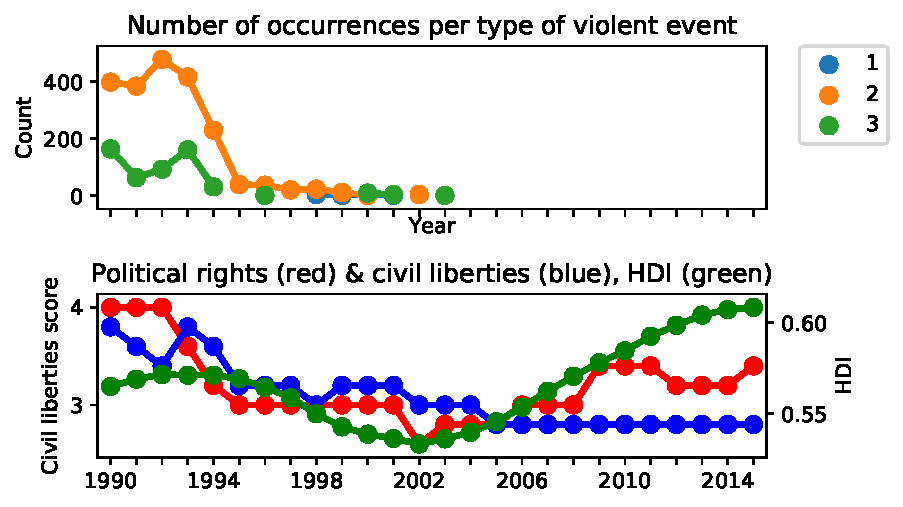
\includegraphics[width=0.50\textwidth]{images/sa.pdf}
    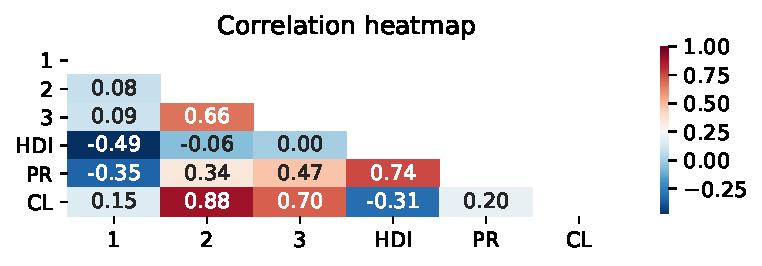
\includegraphics[width=0.50\textwidth]{images/sa_corr.pdf}
\end{figure}

South Africa breaks the pattern that we have observed thus far. HDI, while starting out higher than in both previous regions, is mostly decreasing from 1990 to 2002, but then starts going back up. It correlates most with violence of type 1 ($\rho = -0.49$) which would make sense assuming that less conflict leads to higher life expectancy, better eduction and a higher GDP\@. At the same time, civil liberty and political rights show mostly positive correlations with violence of types 2 and 3, suggesting that more violence of those types lead to higher (worse) scores.

The conflict numbers are almost entirely based on the data from South Africa (country, not region), as the data for the remaining countries is either missing, spotty or insignificant in magnitude. South African countries have been dearly affected by an HIV epidemic in the 90s and early 2000s, which is most likely the reason for the strong downward trend in the HDI curve of that region.

\subsection{West Africa}
\begin{figure}[ht!]
    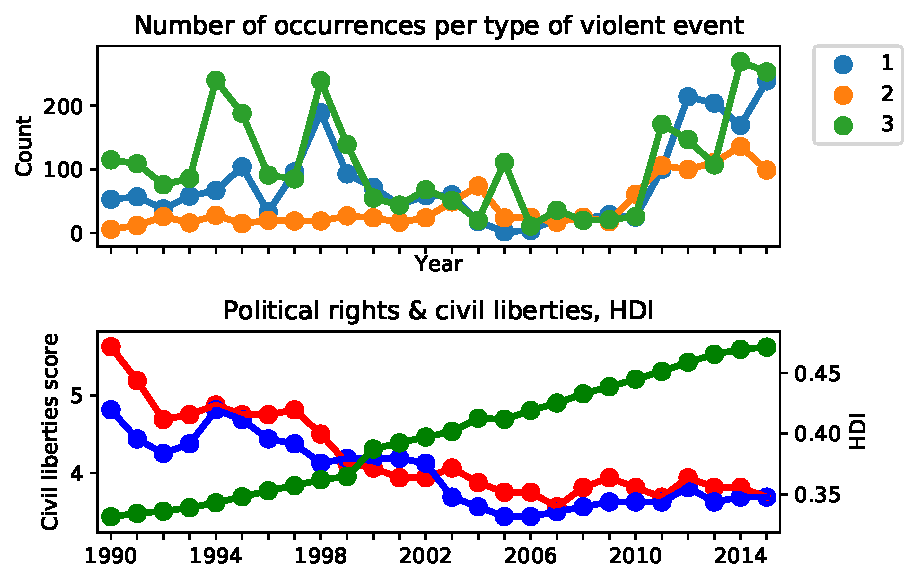
\includegraphics[width=0.50\textwidth]{images/wa.pdf}
    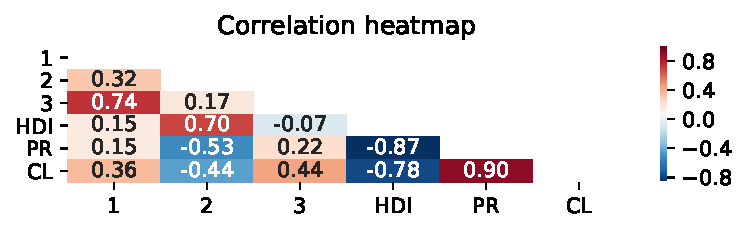
\includegraphics[width=0.50\textwidth]{images/wa_corr.pdf}
\end{figure}
The most apparent connection appears to be between violence of type 2 and all three indicator variables. This is a pattern that we have observed before in North and East Africa: Non state violence coinciding with an improvement in both HDI and civil liberties / political rights. 

We must point out that Nigeria dominates the statistic when it comes violence in this region, especially in recent years with the advent of the terrorist group `Boko Haram' it has seen a sharp rise in state based and one sided violence.

\subsection{Central Africa}
\begin{figure}[ht!]
    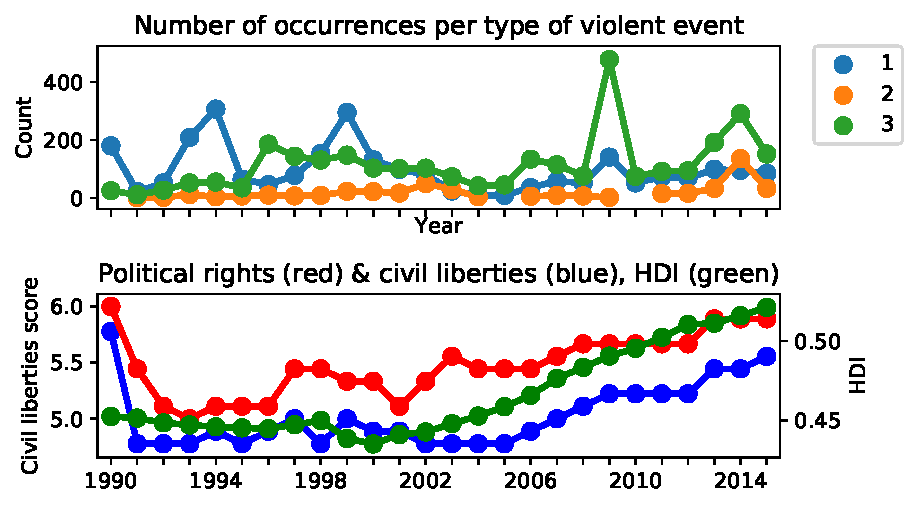
\includegraphics[width=0.50\textwidth]{images/ca.pdf}
    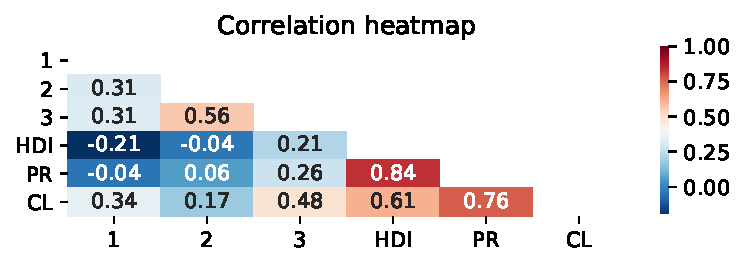
\includegraphics[width=0.50\textwidth]{images/ca_corr.pdf}
\end{figure}
Central African region has experienced high and positive correlation between Human Development Index and both civil rights and political freedom scores, resulting in the improvement in the standard of living while civil liberties have worsened in the same observed period. Moreover, considering that many of the countries in this region are ruled by de facto dictators, who have been holding on to power for decades, these numbers are not very surprising.

The region has been experiencing temporal spikes in the frequency of conflicts due to tribal clashes and government-sanctioned actions against civilians. In the recent history outlier from the year 2009 stands out, originating from the conflicts on the border between Democratic Republic of the Congo and Rwanda. Rwandan military was allowed to cross borders of the Democratic Republic of the Congo in order to pursuit opposing Hutu militatnts, resulting in the now called ‘Kivu conflict’.

\section{Case Study: Zimbabwe}
Zimbabwe is a landlocked eastern African country once seen as a regional economic leader, but since the year 2000 Zimbabwe has struggled to feed its own people due to severe droughts and the effects of a land reform program which saw the seizure of white-owned farms redistributed to landless black Zimbabweans, consequently leading to sharp falls in production. Cash-strapped and impoverished, Zimbabwe's economy faces severe challenges. Unemployment and poverty are endemic and political strife and repression commonplace. Many Zimbabweans have left the country in search of work in South Africa.

Through the observed period from 1990--2015 Zimbabwe has only experienced one-sided violent events, all of whom are reported to include Zimbabwe’s government as the aggressor directly, or indirectly through Renamo. Renamo is Mozambican National Resistance, a militant organization and political movement in Mozambique sponsored by the Rhodesian Central Intelligence Organization.

Both numbers of violent events and casualties sustained experience peak in the year of 2008, during the presidential and parliamentary elections that saw violent clashes between supporters of incumbent president Robert Mugabe, and his challenger Morgan Tsvangirai. Challenger candidate backed out off the run-off round complaining of intimidation and violence against his supporters, and incumbent president consequently won another mandate. These elections will prove to be the start of the decline in Zimbabweans civil liberties that will continue until 2015.

Human development index’s steady decline from the year 1991 to 2000 reflects decline in the Zimbabwean population’s health, where by 1997 an estimated 25\% of the population had been infected by HIV in a pandemic that was affecting most of southern Africa. In 2000, the government pressed ahead with its ‘Fast Track Land Reform’ program, a policy involving compulsory land acquisition aimed at redistributing land from the minority white population to the majority black population. Confiscations of white farmland, continuous droughts, and a serious drop in external finance and other supports led to a sharp decline in agricultural exports, which were traditionally the country's leading export-producing sector. Some 58,000 independent black farmers have since experienced limited success in reviving the gutted cash crop sectors through efforts on a smaller scale. President Mugabe and the ZANU-PF party leadership found themselves beset by a wide range of international sanctions. In 2002, the nation was suspended from the Commonwealth of Nations due to the reckless farm seizures and blatant election tampering.

The Zimbabwe Democracy and Economic Recovery Act of 2001 (ZDERA) went into effect in 2002. ZDERA is an act passed by the United States Congress sanctioned to provide for a transition to democracy and to promote economic recovery in Zimbabwe. This as a result saw Zimbabwe’s human development index to increase steadily from 2002, with slight dip in the year 2008 due to aforementioned unrests during presidential and parliamentary elections.

\section{Conclusion}

Through combination of datasets providing information about frequency and nature of violent events, life expectancy, education level, GDP per capita, and civil and political liberties we were able to obtain robust and relevant picture of the impact that violent events have had on the African civilian population in the period of 1990--2015. Regional exploration observed unique trends further supported by research into regional socio-economic climates, providing support beyond correlation between indicators. Finally, Zimbabwe case study presented possibilities of more granular pursuit into country specific topics based on the sound observations we have made in our earlier work.


%{\bf Citations}: Citations within the text appear in parentheses
%as~\cite{Gusfield:97} or, if the author's name appears in the text
%itself, as Gusfield~\shortcite{Gusfield:97}.  Append lowercase letters
%to the year in cases of ambiguity.  Treat double authors as
%in~\cite{Aho:72}, but write as in~\cite{Chandra:81} when more than two
%authors are involved. Collapse multiple citations as
%in~\cite{Gusfield:97,Aho:72}. Also refrain from using full citations
%as sentence constituents. We suggest that instead of
%\begin{quote}
%  ``\cite{Gusfield:97} showed that ...''
%\end{quote}
%you use
%\begin{quote}
%``Gusfield \shortcite{Gusfield:97}   showed that ...''
%\end{quote}

%If you are using the provided \LaTeX{} and Bib\TeX{} style files, you
%can use the command \verb|\newcite| to get ``author (year)'' citations.
%
%\textbf{References}: Gather the full set of references together under
%the heading {\bf References}. Arrange the references alphabetically
%by first author, rather than by order of occurrence in the text.
%Provide as complete a citation as possible, using a consistent format,
%such as the one for {\em Computational Linguistics\/} or the one in the 
%{\em Publication Manual of the American 
%Psychological Association\/}~\cite{APA:83}.  Use of full names for
%authors rather than initials is preferred.  A list of abbreviations
%for common computer science journals can be found in the ACM 
%{\em Computing Reviews\/}~\cite{ACM:83}.
%
%\subsection{Footnotes}
%
%{\bf Footnotes}: Put footnotes at the bottom of the page and use 9
%points text. They may be numbered or referred to by asterisks or other
%symbols.\footnote{This is how a footnote should appear.} Footnotes
%should be separated from the text by a line.\footnote{Note the line
%separating the footnotes from the text.}
%
%\subsection{Graphics}
%
%{\bf Captions}: Provide a caption for every illustration; number each one
%sequentially in the form:  ``Figure 1. Caption of the Figure.'' ``Table 1.
%Caption of the Table.''  Type the captions of the figures and 
%tables below the body, using 11 point text.


\bibliographystyle{acl}
\bibliography{ada2017}

\end{document}
